
\chapter*{\label{ref-012}Valthe en kleinkinderen}

\begin{figure}[h]
    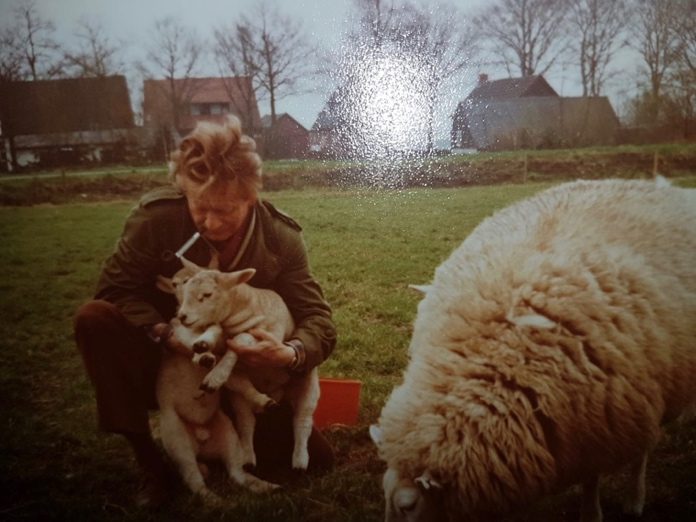
\includegraphics[width=\textwidth]{image56}
    \caption{Met de schapen in Valthe.}
\end{figure}

\begin{figure}[h]
    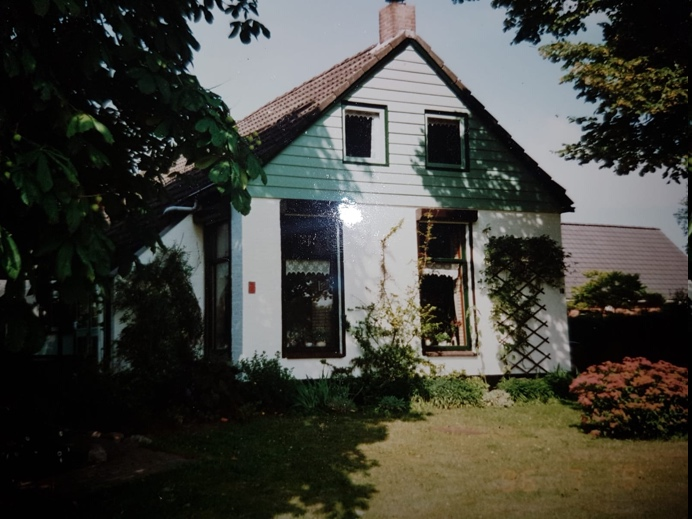
\includegraphics[width=\textwidth]{image57}
    \caption{Het huis in Valthe.}
\end{figure}

\lettrine[lines=2, loversize=0.3, lraise=0]{\initfamily L}{ater} ging Joop met vervroegd pensioen en verhuisden we naar Valthe, zodat er meer ruimte was: 1,5 ha grond. En een verbouwd boerderijtje. Er kwamen schapen en lammetjes, kippen en ganzen. En een moestuin. Dat was wel leuk.

Drenthe is een prachtige provincie. Joop en ik reden een keer door Drenthe en eigenlijk kenden we Drenthe helemaal niet en toen zeiden we tegen elkaar: ``Wat is dit ook een mooie provincie!'' En toen besloten we dus dat we daar best konden gaan wonen. Nou, maar dan vind je natuurlijk niks, h\`{e}. En toen hebben we het uit handen gegeven aan een makelaar en die vond het huis aan de Vlintweg in Valthe. Want Joop had gezegd; ``Ik wil wel ruimte om me heen hebben''. Nou, zei die makelaar, ruimte dat heb je dan wel. 

\begin{figure}[h]
    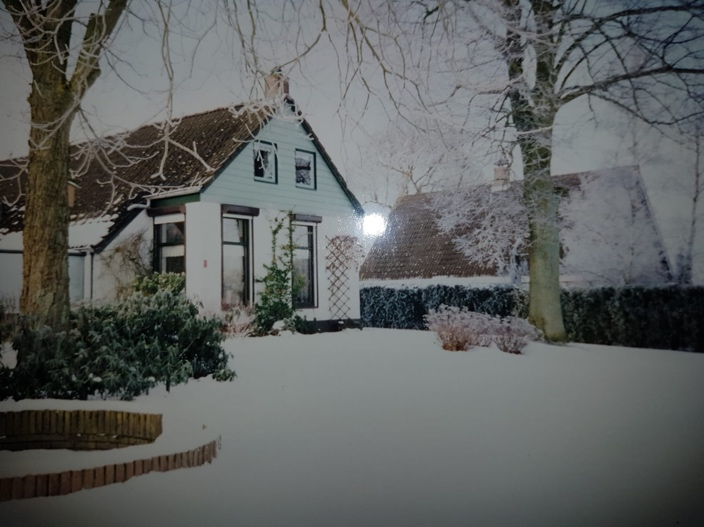
\includegraphics[width=\textwidth]{image58}
    \caption{Het huis in Valthe in de winter.}
\end{figure}

Nou wat moet je daar dan als niet-landbouwer? Er kwam een heel kerstbomenbos en kippen en schapen en een hond. Ook lammetjes werden er geboren in de lente en dan soms moest er \'{e}\'{e}ntje met de fles worden grootgebracht, maar dat vond ik wel leuk, hoor! Zo ging ik op een dag naar het dorp om een zuigfles te kopen! Ja, dat heb ik ook allemaal gedaan...Er zijn ook nog foto’s van. 

Toen de kleinkinderen wat groter waren kwamen ze wel logeren in Valthe. Op zolder was de bedoeling, maar er was ook een logeerkamer beneden, waar ze vaak sliepen. Er was ruimte genoeg!

\begin{figure}[h]
    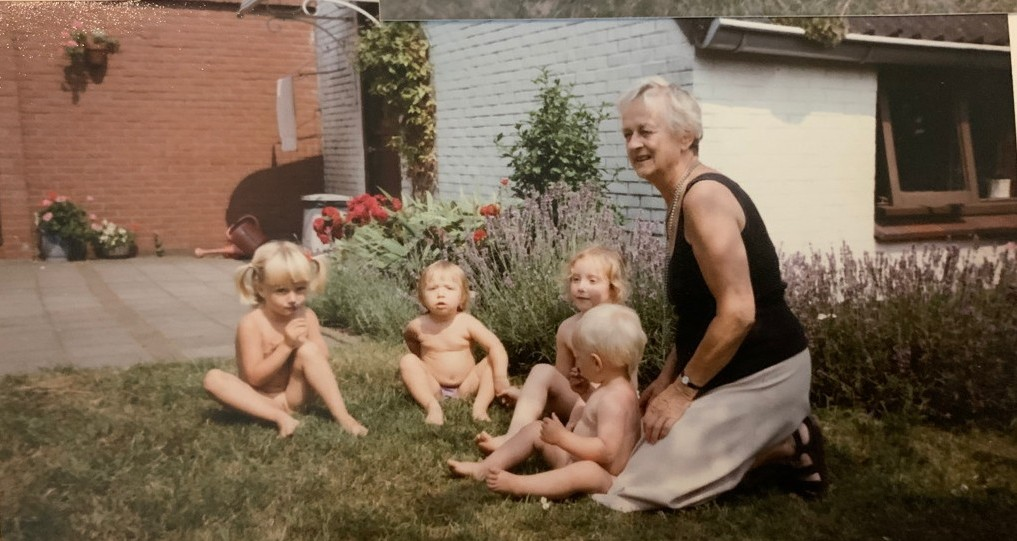
\includegraphics[width=\textwidth]{image59}
    \caption{Met de kleinkinderen achter het huis in Valthe.}
\end{figure}
\begin{figure}[h]
    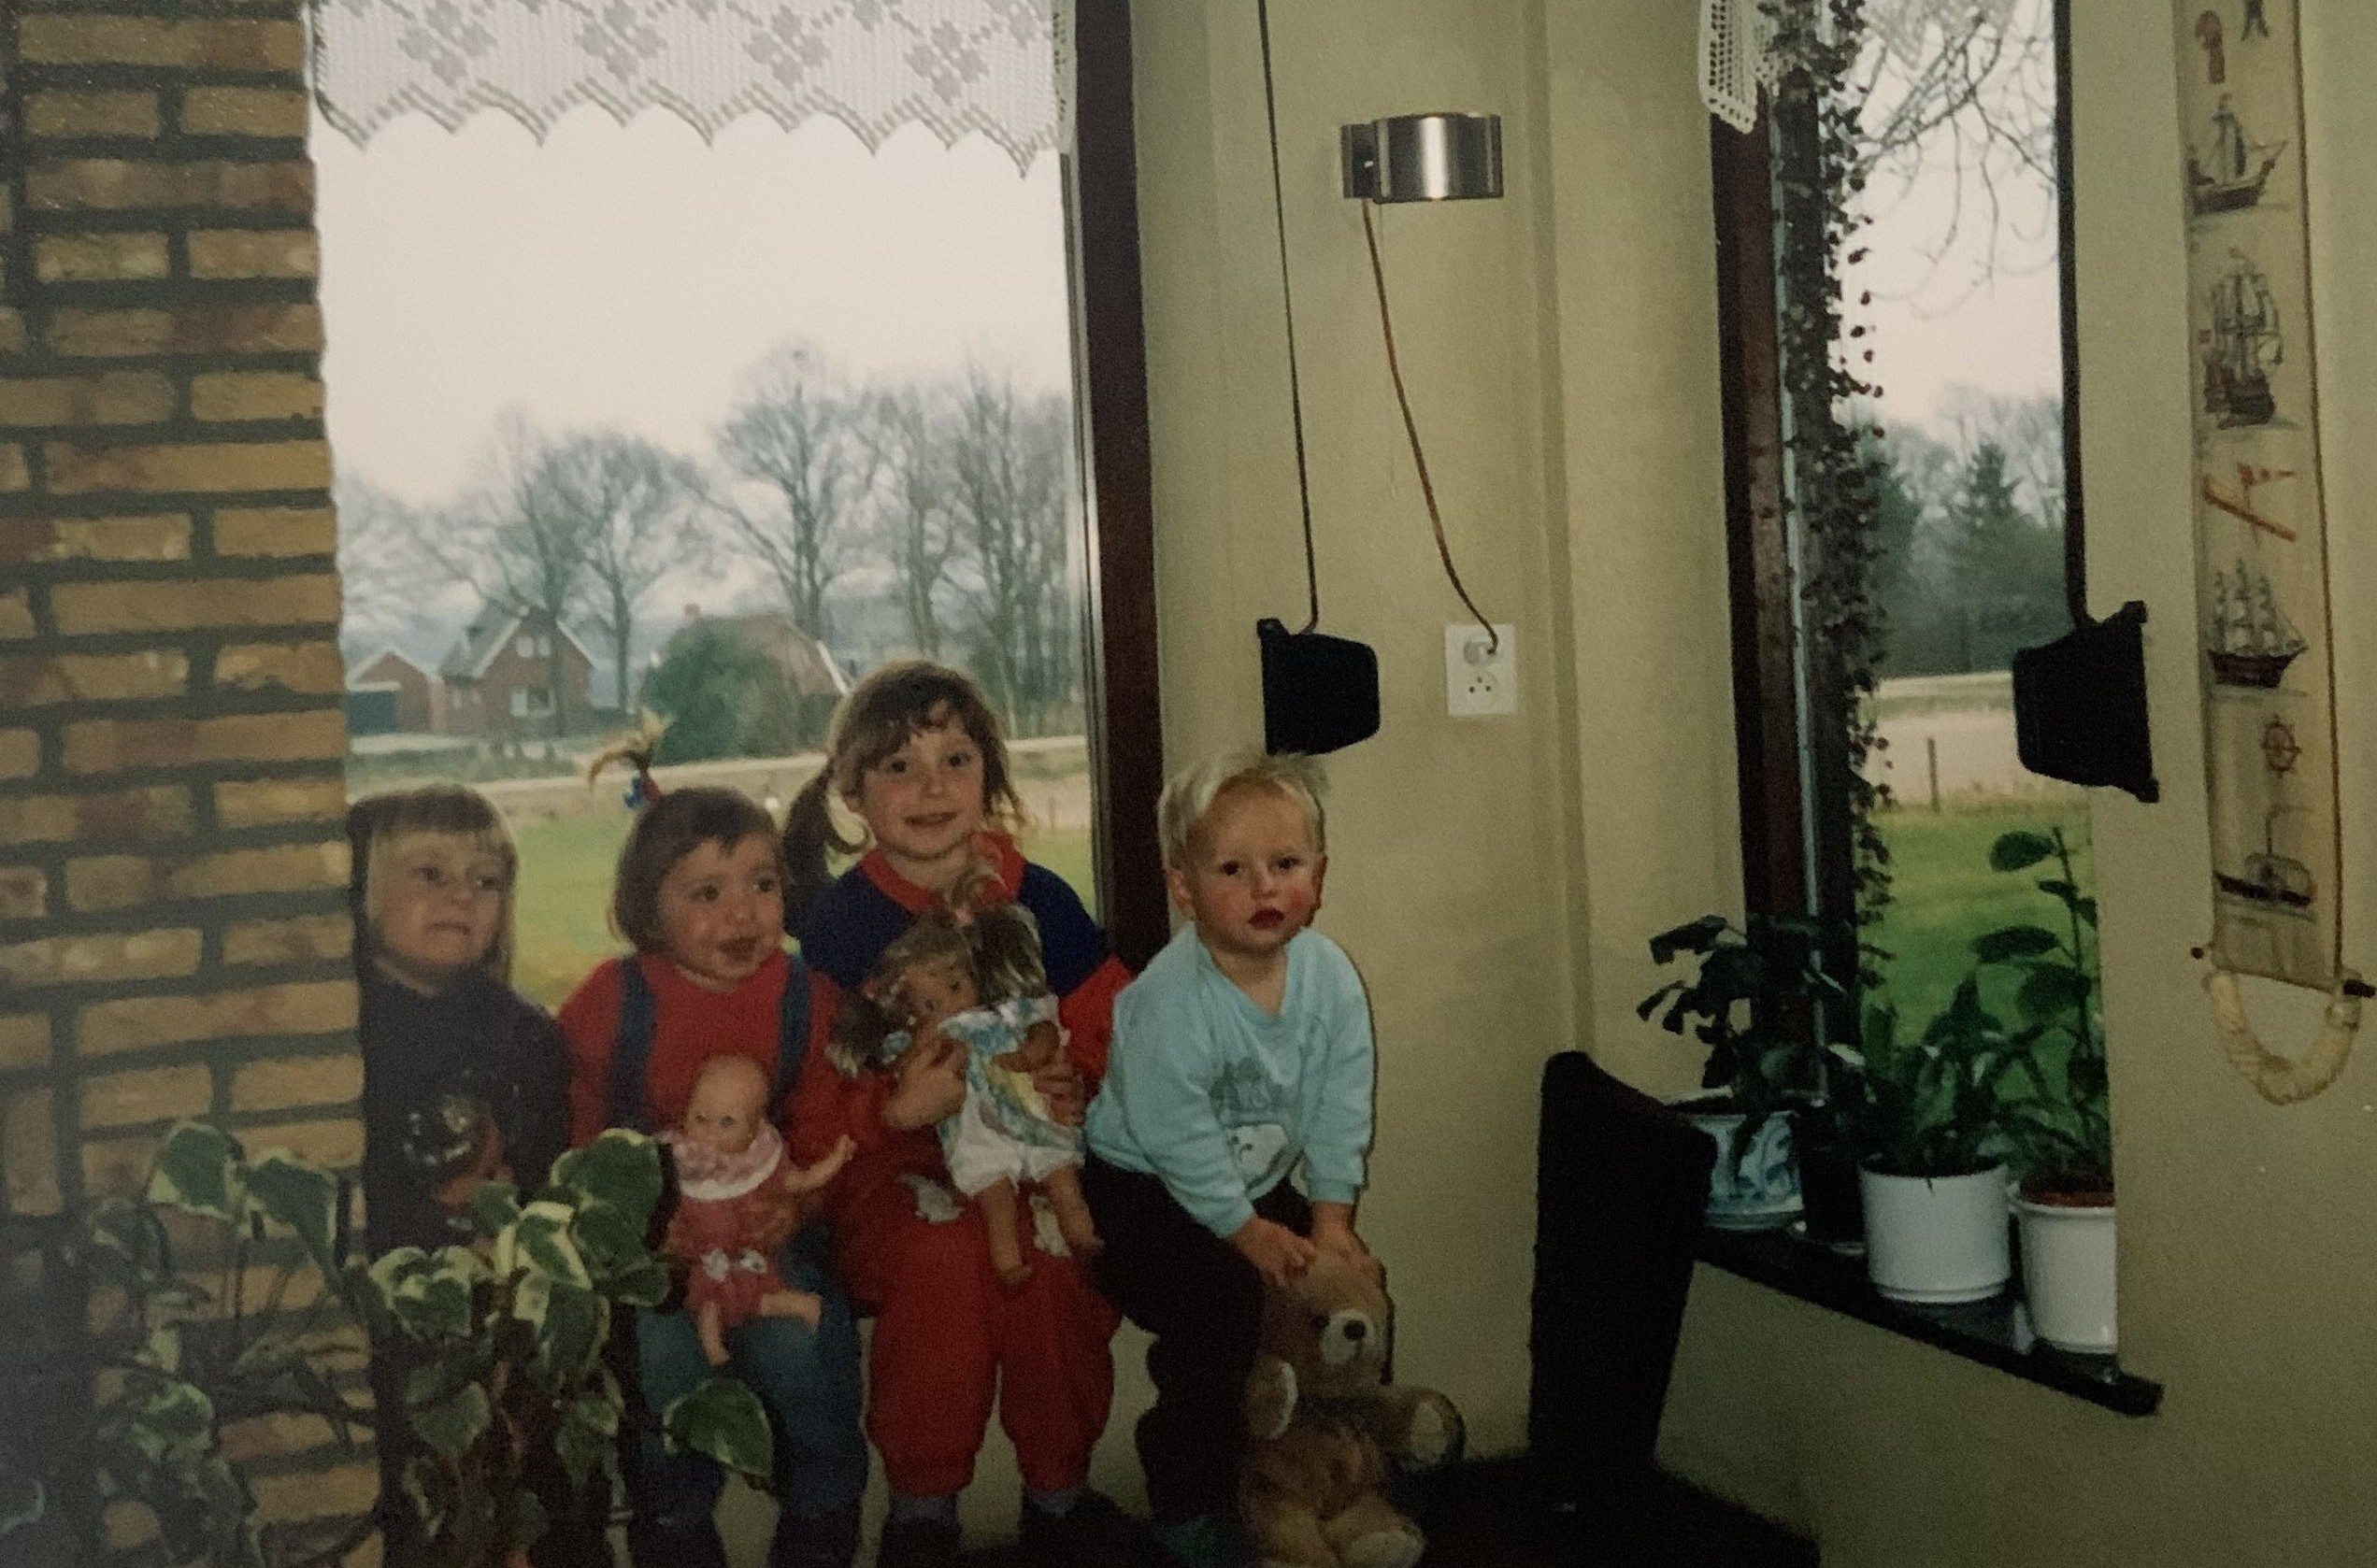
\includegraphics[width=\textwidth]{image60}
    \caption{De kleinkinderen op bezoek.}
\end{figure}

Later werd Joop ziek en ik wist dat hij zou te komen overlijden, dus dan heb je toch mensen om je heen nodig en dat had ik gelukkig. Ik was gaan volksdansen en had een groepje vrouwen, waar ik mee wandelde en fietste. En je moet natuurlijk niet als je alleen komt te staan achter de gordijnen gaan zitten. 

Met de slaaptrein ben ik toen nog naar Frankrijk gegaan om Yvonne en haar gezin op te zoeken. Ik weet nog dat Yvonne fietste met C\'{e}line achterop. Ik had een rieten kinderzitje voor achterop de fiets meegenomen en dat was een hele bezienswaardigheid daar, want niemand had dat!

In die tijd heb ik ook darmkanker gehad, maar ik dacht helemaal niet dat ik eraan dood zou gaan. Ze ontdekten het doordat ik bloed aan de bloedbank gaf, daardoor was ik er op tijd bij. Ja, dat weet ik nog wel. Ik was er niet van ondersteboven. Ik bedoel, dat komt dan op je weg en dan ga je het aan. We zijn toen wel met alle kinderen en kleinkinderen in een huisje een weekendje weggeweest voor de operatie. Nog even genieten.

Tijdens de chemo had ik veel aan de buren. Lucas was een goede buurman en Lammie een goede buurvrouw. Met Lammie heb ik wel veel gefietst maar we hebben nooit een reis gemaakt.